%------------       插入图片的示例   ------------------------------------------
%\begin{center}
%\includegraphics[width=4in]{untitled2.jpg}
%\end{center}
%----------------插入参考文献---------------------------------------
%		\begin{thebibliography}{1}
%		\end{thebibliography}
%<span style="font-size:18px;">\begin{thebibliography}{}
%	\bibitem[显示符号]{引用标签} Book Title, Author
%\end{thebibliography}</span>
%--------------   公式组  vspace 用于调整公式间的距离  ----------------------------
%$$\left\{	\begin{array}{cc}
%\displaystyle\int_{s}^{d} & \int_{s}^{d} \vspace{1ex}\\
%\displaystyle\sum_{d}^{kk} & \int_{s}^{d}
%\end{array}
%\right.$$
%----------------   一组公式 --------------------------------------
%\begin{align*}
%\int_{s}^{d} \vspace{10ex}\\
%\int_{s}^{d}\\
%\int_{s}^{d}
%\end{align*}
%------------------------------------------------------------------
\documentclass[letterpaper,12pt]{article}
\usepackage{indentfirst}
\setlength{\parindent}{2em}
\usepackage{tabularx} % extra features for tabular environment
\usepackage{latexsym,bm}
\usepackage{amsmath,amssymb}  % improve math presentation
\usepackage{cases}
\usepackage{pifont}
\usepackage{setspace}
\usepackage{graphicx, subfig}
\usepackage{float}
\usepackage[margin=1in,letterpaper]{geometry} % decreases margins
\usepackage{cite} % takes care of citations
%\usepackage[final]{hyperref} % adds hyper links inside the generated pdf file
\usepackage{fourier}
\usepackage{xcolor}
\usepackage[english]{babel}
\usepackage{titlesec}
%\usepackage{algorithm}
\usepackage[ruled]{algorithm2e}
\usepackage{algpseudocode}
\usepackage[colorlinks,linkcolor=red]{hyperref}
%\renewcommand{\algorithmicrequire}{\textbf{Input:}}  % Use Input in the format of Algorithm
%\renewcommand{\algorithmicensure}{\textbf{Output:}} % Use Output in the format of Algorithm

\titleformat{\section}[block]{\Large\bfseries\filcenter}{\thesection .}{1em}{}
%\titleformat{\subsection}[block]{\medium\bfseries\filcenter}{\thesection .}{1em}{}
\usepackage[UTF8]{ctex}
\renewcommand{\baselinestretch}{1.5}        % 定义行距
%\setlength{\abovedisplayskip}{2pt plus1pt minus1pt}     %公式前的距离
%\setlength{\belowdisplayskip}{6pt plus1pt minus1pt}     %公式后面的距离
\setlength{\arraycolsep}{2pt}   %在一个array中列之间的空白长度, 因为原来的太宽了
\allowdisplaybreaks[4] % \eqnarray如果很长,影响分栏、换行和分页
                        %(整块挪动,造成页面空白),可以设置成为自动调整模式
\setlength\jot{9pt} %调整多行公式之间的距离

\hypersetup{
	colorlinks=true,       % false: boxed links; true: colored links
	linkcolor=blue,        % color of internal links
	citecolor=blue,        % color of links to bibliography
	filecolor=magenta,     % color of file links
	urlcolor=blue
}
%++++++++++++++++++++++++++++++++++++++++
\begin{document}
\title{Particle filter based template matching}
\author{谢翠芳}
\date{\today}
\maketitle


\section{Experiment condition}

The aim of this experiment is to make sure the idea of combining particle filter and template matching is possible. 'Possible' means we can match the template with targets in limited number of points and iterations. All we have is a target's template and an image. The template is curved directly from the image. And the image includes the target because of the experiment aim.

We tested the above method in two couples of templates and images. One image has size of 960*448, the other has the size of 360*240. And the result of the 960*448 sized image will be discussed in detail.


\section{Method}

\begin{enumerate}
\item Sample points in the image, and calculate the feature for the certain number of sampled points.
\item Arrange weights for the sampled points according to the distance between features of the template and the points.
\item Re-sample same number of points according to the points' weights.
\item Repeat the above steps several times(the iteration depends on the number of sampled points).
\end{enumerate}

The complexity of the method mainly depends on the number of sampled points and the iteration times. While the iteration times depend on the number of sampled points.

\section{Results of the 960*448 image}

The matching feature is color histogram for all experiments.

When iteration is 5, do the same experiment for 10 times. The number of right-matching versus with number of sampled points.

\begin{figure}[H]
\centering%图片居中
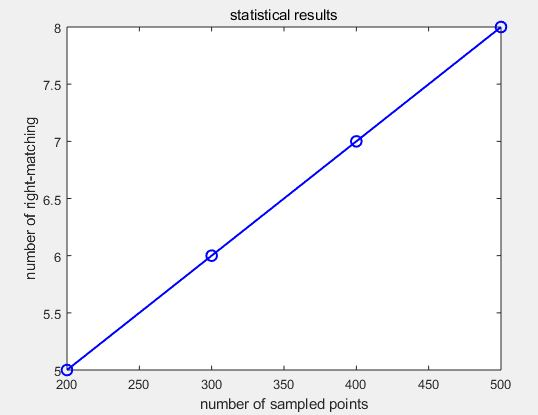
\includegraphics[width=5in]{iterationD.jpg}
\caption{right-matching versus number of points}
\label{Fig.1}
\end{figure}

From figure 1, it is obvious that the number of right matching increases along with the number of sampled points.

When number of sampled points is 300, do the same experiment for 10 times. The number of right-matching versus with number of iteration.

\begin{figure}[H]
\centering%图片居中
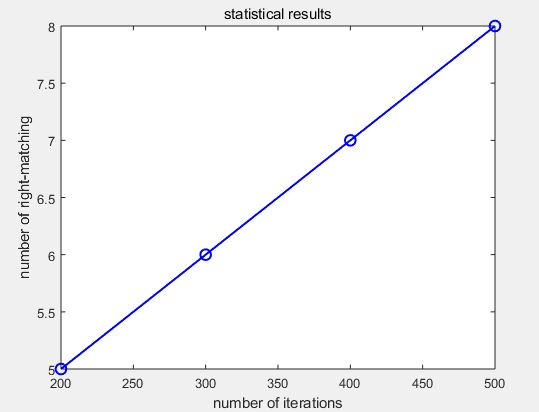
\includegraphics[width=5in]{pointD.jpg}
\caption{right-matching versus number of iteration}
\label{Fig.2}
\end{figure}

Figure 2 shows that the number of right matching increases if iteration times increase.

Figure 1 and figure 2 show like the number of right matching and the number of sampled points(or iterations) are proportional. And when the number of sampled points is large enough, the probability of right-matching is high.

The raw results are in the appendix.

\section{Unsolved problems}

\begin{enumerate}
  \item The size of template and image target should be similar in the experiment. Next step, different size template and preprocessing of images should be considered. And preprocessing
  \item How to decide the number of particles? After solving the 'size problem', particle number will be considered. Especially the relationship with the size of template and size of images.
  \item Threshold of judging whether there is a target is not discussed in this experiment.
  \item Feature used for calculating the distance between template and image is capable to be chosen. So the influence of features should also be discussed in following experiments.

\end{enumerate}

\section{Appendix}

The details of the image match are enlarged.

\begin{figure}[H]
\centering%图片居中
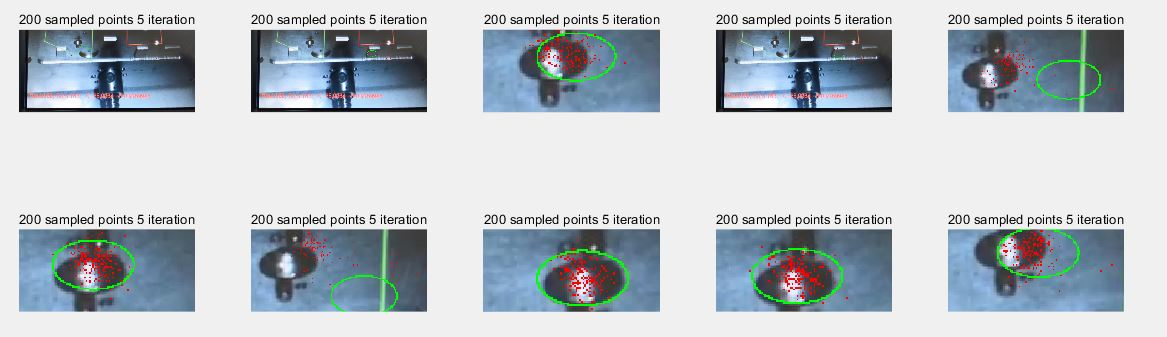
\includegraphics[width=5in]{200n5icompare.jpg}
\caption{number of right matching with 200 particles and 5 iterations}
\label{Fig.3}
\end{figure}

\begin{figure}[H]
\centering%图片居中
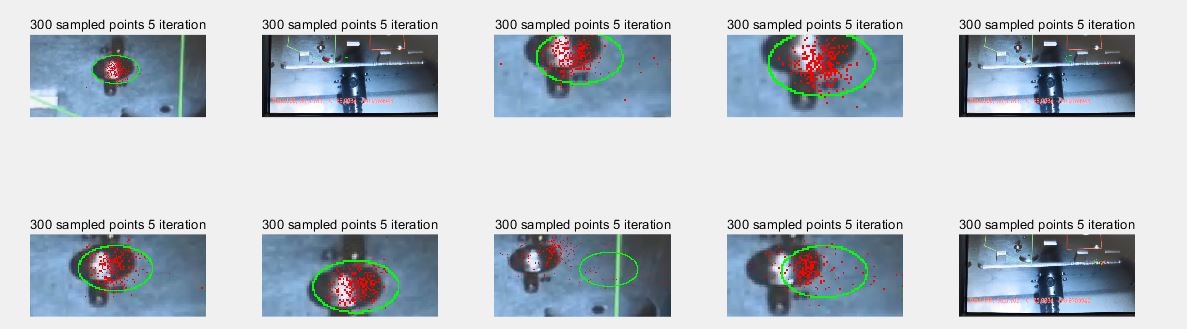
\includegraphics[width=5in]{300n5icompare.jpg}
\caption{number of right matching with 300 particles and 5 iterations}
\label{Fig.4}
\end{figure}


\begin{figure}[H]
\centering%图片居中
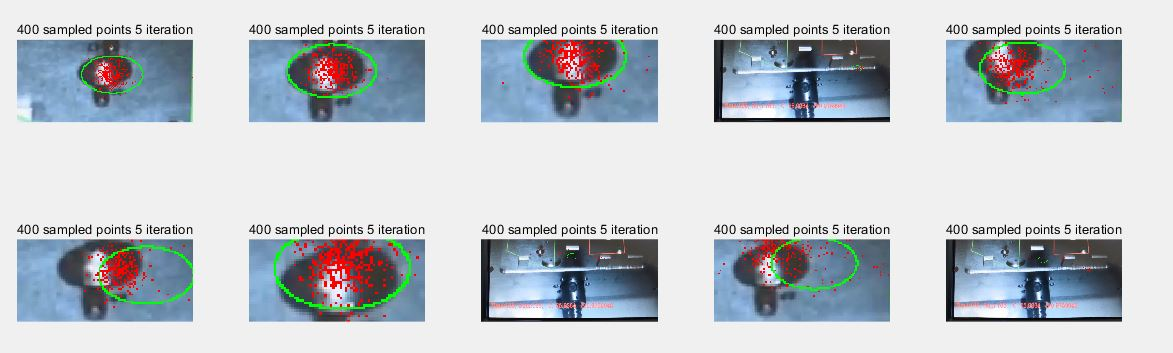
\includegraphics[width=5in]{400n5icompare.jpg}
\caption{number of right matching with 400 particles and 5 iterations}
\label{Fig.5}
\end{figure}


\begin{figure}[H]
\centering%图片居中
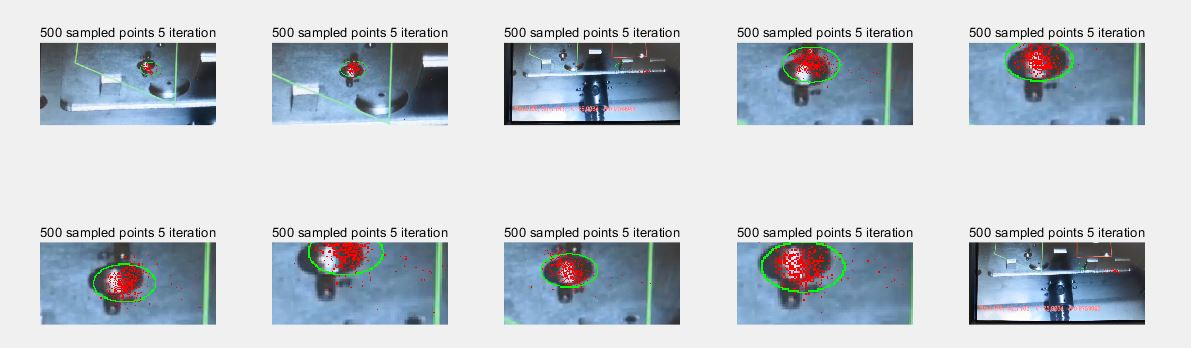
\includegraphics[width=5in]{500n5icompare.jpg}
\caption{number of right matching with 500 particles and 5 iterations}
\label{Fig.6}
\end{figure}


\begin{figure}[H]
\centering%图片居中
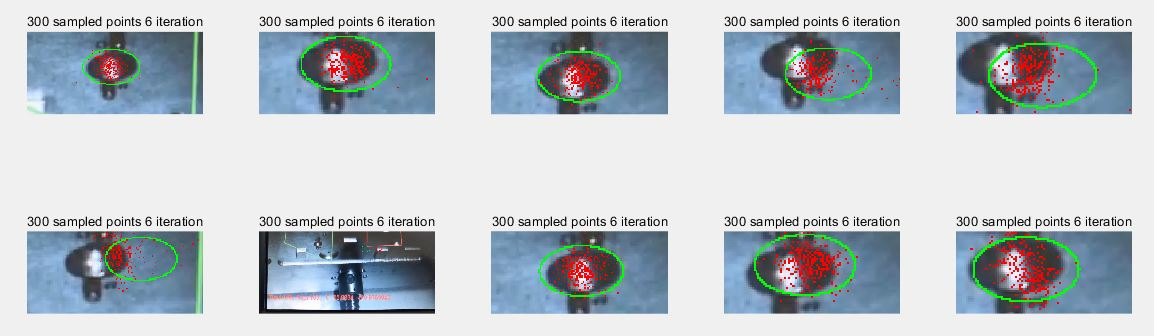
\includegraphics[width=5in]{300n6i.jpg}
\caption{number of right matching with 300 particles and 6 iterations}
\label{Fig.8}
\end{figure}


\begin{figure}[H]
\centering%图片居中
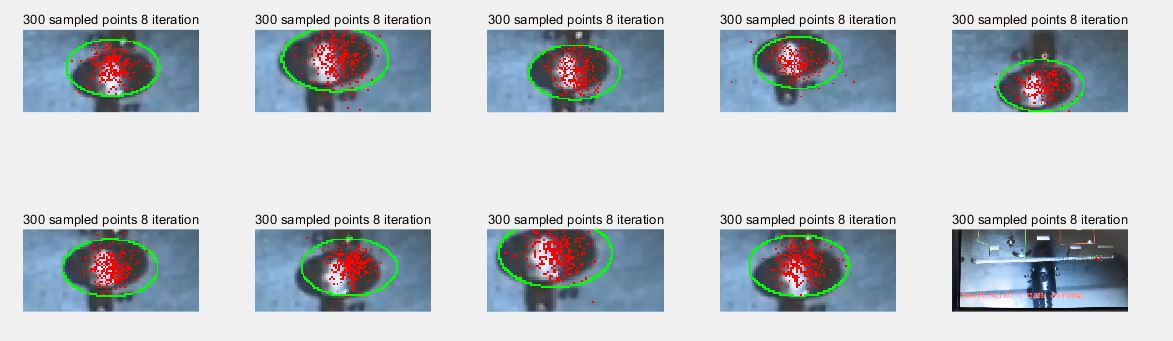
\includegraphics[width=5in]{300n8icompare.jpg}
\caption{number of right matching with 300 particles and 8 iterations}
\label{Fig.9}
\end{figure}


\begin{figure}[H]
\centering%图片居中
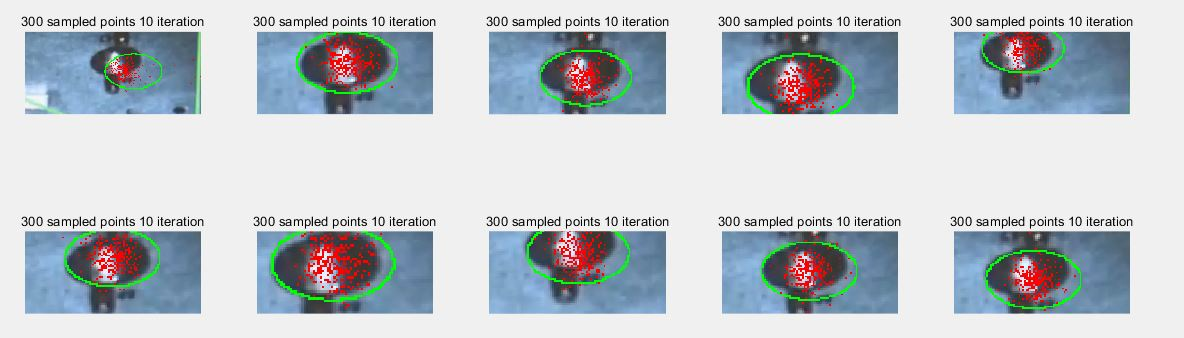
\includegraphics[width=5in]{300n10icompare.jpg}
\caption{number of right matching with 300 particles and 10 iterations}
\label{Fig.10}
\end{figure}


\end{document} 